\section{Auswertung}
\label{sec:Auswertung}
\subsection{Bestimmung der Dichte}
Um die nachfolgend berechneten Elastizitätsmoduln mit Literaturwerten vergleichen
zu können, wird zunächst die Dichte der Stäbe bestimmt. Mit Hilfe einer Tabelle
wird dann das Metall oder die Legierung bestimmt.
Für Stab 1, der eine quadratische Querschnittsfläche hat, wurden folgende
geometrische Abmessungen bestimmt:
\begin{align*}
  \text{Länge } l_1 &= \SI{0.60}{\meter}\\
  \text{Breite } a &= \SI{0.01}{\meter}\\
  \text{Masse } m_1 &= \SI{0.5025}{\kilo\gram}.\\
  \intertext{Für Stab 2 mit einer runden Querschnittsfläche wurde}
  \text{Länge } l_2 &= \SI{0.60}{\meter}\\
  \text{Durchmesser } d &= \SI{0.01}{\meter}\\
  \text{Masse } m_2 &= \SI{0.5025}{\kilo\gram}
\end{align*}
gemessen. Alle Messungen wurden dabei zehn Mal durchgeführt, um den Fehler des
Mittelwerts bestimmen zu können, da jedoch immer der gleiche Wert gemessen wurde,
ist der Fehler 0.
Die Dichte der Probestäbe wird mit
\begin{equation}
  \rho = \frac{m}{V}
  \label{eqn:dichte}
\end{equation}
bestimmt.
Für die gemessene Dichte des quadratischen Stabes folgt
\begin{equation*}
  \rho_1 = \frac{m_1}{l_1 a^2} = \frac{\SI{0.5025}{\kilo\gram}}{\SI{0.60}{\meter}
  (\SI{0.01}{\meter})^2} = \SI{8375}{\kilo\gram \per \cubic\meter}
  \label{eqn:dichte_stab1}
\end{equation*}
und für die des runden Stabes
\begin{equation*}
  \rho_2 = \frac{m_2}{\pi \left(\frac{d}{2}\right)^2 l_2}
  = \frac{\SI{0.3605}{\kilo\gram}}{\pi \left(\SI{0.005}{\meter}\right)^2 \SI{0.55}{\meter}}
  = \SI{8346}{\kilo\gram \per \cubic\meter}.
  \label{eqn:dichte_stab2}
\end{equation*}

Dies entspricht im Rahmen der relativen Fehler von $\Delta \rho_1 = \SI{0.3}{\percent}$
und $\Delta \rho_2 = \SI{0.6}{\percent}$ der literaturbekannten Dichte von Messing
(\cite[274]{geschke}, Tabelle 1: Einige Eigenschaften fester Stoffe) und legt nahe,
dass die Stäbe aus Messing sind. Für eine Messing-Legierung mit einer Zusammensetzung
von $\SI{60}{\percent}$ Kupfer und $\SI{38}{\percent}$ Zink ist dort eine Dichte
von $\rho_{Messing}=\SI{8400}{\kilo\gram \per \cubic\meter}$ angegeben.

\subsection{Flächenträgheitsmomente}
\label{sec:Flaechentraegeitsmoment}
Für die Berechnung des Elastizitätsmoduls werden die Flächenträgheitsmomente der
verschiedenen Stäbe benötigt. Das Flächenträgheitsmoment $I$ wird mit der Gleichung
(xx) berechnet.
\subsubsection{quadratischer Stab}
Für den Stab mit quadratischer Querschnittsfläche und einer Kantenlänge von
$h = \SI{0.01}{\meter}$ ergibt sich
\begin{equation}
  I_1 = \int_{-\frac{h}{2}}^{\frac{h}{2}} \int_{-\frac{h}{2}}^{\frac{h}{2}}
  y^2 \symup{d}x \symup{d}y
  = h \cdot \left[\frac{1}{3} y^3\right]_{-\frac{h}{2}}^{\frac{h}{2}}
  = \frac{h^4}{12} = \SI{8.33e-10}{\meter\tothe{4}}.
  \label{eqn:I_quadratisch}
\end{equation}
\subsubsection{runder Stab}
Weiter ergibt sich für den Stab mit runder Querschnittsfläche und dem Radius
$R=\frac{d}{2}=\SI{0.005}{\meter}$ unter Verwendung der Polarkoordinaten
$
\begin{pmatrix}
  x \\
  y
\end{pmatrix}
=
\begin{pmatrix}
  r \sin\varphi \\
  r \cos\varphi
\end{pmatrix}
$
\begin{equation}
  \begin{split}
  I_2 &= \int_0^{2\pi} \int_0^R r \cdot r^2 \cos^2\!\varphi\, \symup{d}r \symup{d}\varphi
  =\frac{R^4}{4}\left[\frac{1}{2}(\varphi + \underbrace{\sin\varphi \cos\varphi}_{=0})\right]_0^{2\pi} \\
  &=\frac{\pi R^4}{4} = \SI{4.91e-10}{\meter\tothe{4}}
  \end{split}
  \label{eqn:I_rund}
\end{equation}


\subsection{Einseitige Einspannung}
\subsubsection{eckiger Stab}
Die zur Berechnung der Durchbiegung $D(x)$ nach Gleichung (xx) notwendigen Messwerte
sind in Tabelle \ref{tab:messung1} dargestellt, welche sich zur besseren Lesbarkeit
des Textes im Anhang befindet (sowie alle weiteren Messwerte).\newline
Der Abstand des Messpunktes vom Einspannungspunkt ist $x$, $D_0(x)$ ist die
Durchbiegung ohne Belastung des Stabes und $D_M(x)$ die Durchbiegung des Stabes
nach Anhängen eines Gewichts der Masse $M_{G1} = \SI{1.0205}{\kilo\gram}$. Die
effektive Länge des Stabes vom Einspannungspunkt bis zum freien Ende des Stabes
beträgt $l_\text{eff} = \SI{0.49}{\meter}$.

Der Elaztizitätsmodul wird durch eine lineare Ausgleichsrechnung bestimmt. Dazu
wird $D(x)$ gegen $L x^2 - \frac{x^3}{3}$ aufgetragen und mit Python eine lineare
Regression der Form $f(x) = a \cdot x + b$ durchgeführt, welche für die Parameter
$a$ und $b$ die folgenden Werte liefert (siehe dazu Abbildung
\ref{fig:plot_einseitig1}):
\begin{figure}
  \centering
  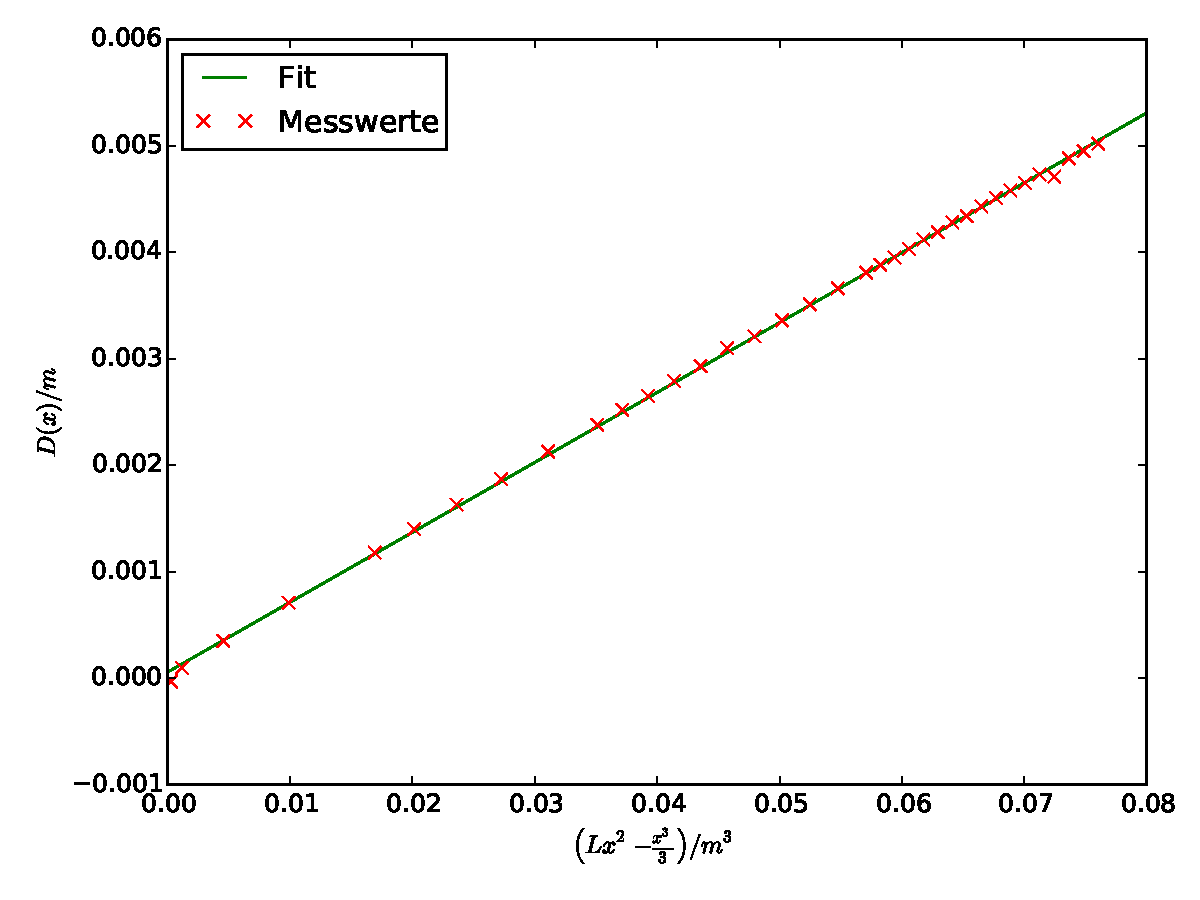
\includegraphics[width=0.9\textwidth]{stab1_einseitig.pdf}
  \caption{Lineare Ausgleichsrechnung für den einseitig eingespannten eckigen Stab.}
  \label{fig:plot_einseitig1}
\end{figure}
\begin{align*}
  a &= \SI{0.06566(23)}{\per\squared\meter} \\
  b &= \SI{0.57(12)e-3}{\meter}.
\end{align*}

Nach Gleichung (xx) wird der Elastizitätsmodul dann mit
\begin{equation}
  a = \frac{F}{2 E I_1} \iff E = \frac{F}{2 I_1 a}
  \label{eqn:Emodul1}
\end{equation}
bestimmt. Dabei ist $I_1$ das in Abschnitt \ref{sec:Flaechentraegheitsmoment}
berechnete Flächenträgheitsmoment. Für den

\subsubsection{runder Stab}


\subsection{Beidseitige Einspannung}
